\documentclass{report}
\usepackage{mathtools}
\usepackage{unicode-math}
\usepackage{lualatex-math}
\usepackage{tcolorbox}
\setmainfont[
  BoldFont={STIXTwoText-Bold},
  ItalicFont={STIXTwoText-Italic},
  BoldItalicFont={STIXTwoText-BoldItalic}
]{STIXTwoText-Regular}
\setmathfont{STIXTwoMath-Regular}

\usepackage{mathdots}

\setlength{\parindent}{0pt}
\setlength{\parskip}{0.5em}

\usepackage{biblatex}
\addbibresource{references.bib}
\usepackage{amsmath}
\usepackage{listings}
\lstset{
  basicstyle=\ttfamily,
  mathescape
}

\renewcommand{\chaptername}{Poglavje}

\DeclareMathOperator{\acc}{symbol}

\usepackage{mathtools}
\usepackage{tikz}
\usetikzlibrary{automata, arrows.meta, positioning, arrows, fit, matrix, shapes.geometric, shapes.misc, calc}
\pgfdeclarelayer{background}
\pgfdeclarelayer{foreground}
\pgfsetlayers{background,main,foreground}

\newcounter{example}
%\newcommand{\N}[1]{{{#1}_{\arabic{example}}}}
\newcommand{\N}[1]{#1}
\newcommand{\Next}{\stepcounter{example}}
\newcommand{\Reset}{\setcounter{example}{1}}

\newcommand{\Ex}{\textbf{Npr.}:\ }
\newcommand{\Special}[1]{\textbf{#1}}
\newcommand{\Empty}{\varnothing}
\newcommand{\Null}{\varepsilon}
\newcommand{\Alphabet}{\Sigma}
\newcommand{\Language}[1]{\mathcal{L}(#1)}
\newcommand{\Automaton}[1]{\mathcal{M}(#1)}
\newcommand{\Str}[1]{\text{\textquotedbl\texttt{#1}\textquotedbl}}
\newcommand{\Char}[1]{\texttt{#1}}
\newcommand{\Seq}{\cdot}
\newcommand{\Pos}{\mathop{\mdsmblkcircle}}
\newcommand{\Spc}{\ }
\newcommand{\Union}{\mathrel{|}}
\newcommand{\Sum}{\mathrel{+}}
\newcommand{\Kleene}[1]{{#1}^\ast}
\newcommand{\Rep}[2]{{#1}^{#2}}
\newcommand{\Opt}[1]{#1?}
\newcommand{\KleenePlus}[1]{#1^+}
\newcommand{\Err}{\rdiagovfdiag}

\newcommand{\Set}[1]{#1}

\newcommand{\FIRST}{\textsc{first}}
\newcommand{\FOLLOW}{\textsc{follow}}
\newcommand{\NEXT}{\textsc{next}}
\newcommand{\EOF}{\textsc{eof}}
\newcommand{\Terminals}{\Set{T}}
\newcommand{\Productions}{\Set{P}}
\newcommand{\NonTerminals}{\Set{N}}

\newcommand{\Arrow}{\Coloneq}
\newlength{\arrow}
\settowidth{\arrow}{\scriptsize$000$}
\newcommand{\MoveX}[1]{\xrightarrow{\mathmakebox[\arrow]{#1}}}
\newcommand{\Move}{\MoveX{}}
\newcommand{\MoveStar}{\nolinebreak\mathrel{\Move\!\!{}^\ast}\nolinebreak}
\newcommand{\Derive}{\Rightarrow}
\newcommand{\DeriveStar}{\Rightarrow^\ast}
\newcommand{\DerivePlus}{\Rigtharrow^+}

\newcommand{\NT}[1]{{#1}}
\newcommand{\T}[1]{{#1}}
\newcommand{\Var}[1]{{#1}}
\newcommand{\Sym}[1]{{#1}}
\newcommand{\RE}[1]{{#1}}
\newcommand{\Lookahead}[1]{{}_{\{{#1}\}}}

\makeatletter
\DeclareRobustCommand{\Dots}{%
  \vbox{
    \baselineskip4\p@\lineskiplimit\z@
    \kern-\p@
    \hbox{.}\hbox{.}\hbox{.}
  }}
\makeatother

\lstnewenvironment{algorithm}[1][]
{
    \lstset{
        mathescape=true,
        %frame=tB,
        numbers=left, 
        %numberstyle=\tiny,
        basicstyle=\footnotesize, 
        %keywordstyle=\color{black}\bfseries\em,
        keywords={,input, output, return, datatype, function, in, if, else, foreach, while, begin, end, } 
        numbers=left,
        xleftmargin=.04\textwidth,
        #1
    }
}
{}

\tikzset{
    cross/.pic = {
    \draw[rotate = 45] (-#1,0) -- (#1,0);
    \draw[rotate = 45] (0,-#1) -- (0, #1);
    },
    hide/.style={draw=none, fill=none},
    ellip/.append style={ellipse, inner sep=-0.14cm},
    every state/.append style={font=\footnotesize},
}

\begin{document}

\chapter{Končni avtomati}

\section{Jezik}
Jezik je (ne nujno končna) množica nizov.

\Ex
\begin{equation*}
  L = \{\Str{}, \Str{DoberDan}, \Str{123}, \Str{/}, \Str{1 + 1} \}
\end{equation*}

\section{Regularni izrazi}
Regularni izrazi so algebra nad jeziki, ki sestavljena iz osnovnih operacij $(\Union)$, $(\Seq)$, $(\ast)$ in osnovnih elementov $\Char{a}$, $\Empty$, $\Null$.
Z njimi lahko opišemo le podmnožico vseh jezikov, ki se imenuje "regularni jeziki".
Dva regularna izraza sta enaka, če opisujeta enak jezik.

\section{Končni avtomati}

Končni avtomat je tuple $(Q, \Alphabet, \delta, q_0, F)$, kjer je $Q$ končna množica stanj, $\Sigma$ končna množica znakov ali abeceda, $\delta$ je funkcija prehodov in $F$ končna množica končnih stanj.
Tuple lahko implementiramo kot \emph{struct} ali \emph{record}.
Funkcija prehodov ima signaturo $Q \times \Sigma \not\rightarrow Q$.
Implementiramo jo lahko, kot asociativni seznam, iskalno drevo ali tabelo.

\Special{Meta:} Avtomat regularnega izraza $r$ bo označen kot $\Automaton{r}$.

\Special{Meta:} Simbol $\Err$ označuje neveljavno stanje.

\Ex
\begin{equation}
  r_1 = \Kleene{(\Char{b} \Seq (\Char{a} \Spc \Char{b})?)} \Seq \Char{c} \\
\end{equation}
\begin{align*}
  \Automaton{r_1} &= (Q_1, \Sigma, \delta_1, q_{0, 1}, F_1)\\[1em]
  Q_1 &= \{1, 2, 3\} \\[1em]
  \Sigma &= \{\Char{a}, \Char{b}, \Char{c}\} \\[1em]
  \delta_1(1, \Char{b}) & =  2\\
  \delta_1(2, \Char{a}) & =  1\\
  \delta_1(2, \Char{b}) & =  2\\
  \delta_1(2, \Char{b}) & =  3\\[1em]
  q_{0, 1} &= 1 \\[1em]
  F_1 &= \{3\}
\end{align*}

\begin{center}
\begin{tabular}{ | c | c | c | c | }
   \hline
   $\delta_1$ & \Char{a} & \Char{b} & \Char{c} \\
   \hline
  1 & $\Err$ & 2 & $\Err$  \\
   \hline
  2 & 1 & 2 & 3  \\
   \hline
  3 & $\Err$ & $\Err$ & $\Err$   \\
   \hline
\end{tabular}
\end{center}

\begin{center}
  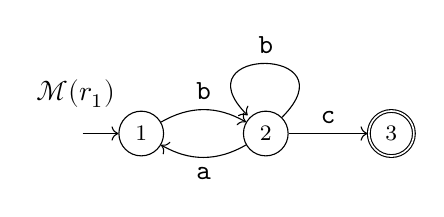
\begin{tikzpicture}
    \tikzset{
      node distance=1cm,
      every state/.append style={minimum size=0.5cm},
      initial text=$ $
    }

    \node[state, initial, label=above left:$\Automaton{r_1}$] (s0) {1};
    \node[state, right=of s0] (s1) {2};
    \node[state, accepting, right=of s1] (s2) {3};

    \draw (s0) edge[->, bend left] node[auto]{$\Char{b}$} (s1);
    \draw (s1) edge[->, bend left] node[auto]{$\Char{a}$} (s0);
    \draw (s1) edge[->, loop] node[above]{$\Char{b}$} (s1);
    \draw (s1) edge[->] node[auto]{$\Char{c}$} (s2);
  \end{tikzpicture}
\end{center}

\Ex

Vsak regularni izraz lahko ustreza večim različnim avtomatom.

\begin{gather*}
  r_2 = \Kleene{(\Char{b} \Seq (\Char{a} \Spc \Char{b})?)} \Seq \Char{c} \\
  \Automaton{r_2} = (Q_2, \Sigma, \delta_2, q_{0, 2}, F_2)
\end{gather*}

\begin{center}
  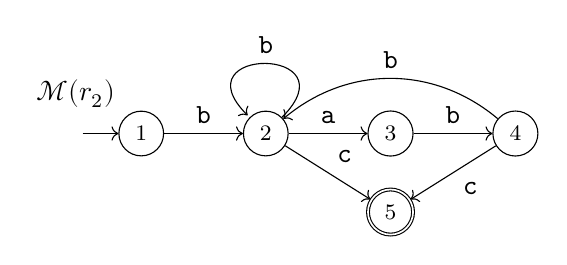
\begin{tikzpicture}
    \tikzset{
      node distance=1cm,
      every state/.append style={minimum size=0.5cm},
      initial text=$ $
    }

    \node[state, initial, label=above left:$\Automaton{r_2}$] (s0) {1};
    \node[state, right=of s0] (s1) {2};
    \node[state, right=of s1] (s2) {3};
    \node[state, right=of s2] (s3) {4};
    \node[state, accepting, below=0.4cm of s2] (s4) {5};

    \draw (s0) edge[->] node[auto]{$\Char{b}$} (s1);
    \draw (s1) edge[->, loop] node[above]{$\Char{b}$} (s1);
    \draw (s1) edge[->] node[auto]{$\Char{a}$} (s2);
    \draw (s2) edge[->] node[auto]{$\Char{b}$} (s3);
    \draw (s1) edge[->] node[auto]{$\Char{c}$} (s4);
    \draw (s3) edge[->] node[auto]{$\Char{c}$} (s4);
    \draw (s3) edge[->, bend right=40] node[above]{$\Char{b}$} (s1);
  \end{tikzpicture}
\end{center}

Funkcijo prehodov lahko definiramo tudi za niz:
\begin{align*} % XXX define empty string
  \Kleene{\delta}(q, \varepsilon) &= q\\
  \Kleene{\delta}(q, a \Seq w) &= \Kleene{\delta}(q', w) \text{, kjer } q' = \delta(q, a) \text{ in } q' \neq \Err
\end{align*}

\Ex
\begin{align*}
  \Kleene{\delta_1}(1, \Str{b}) &= 2 \\
  \Kleene{\delta_1}(1, \Str{ba}) &= 1 \\
  \Kleene{\delta_1}(1, \Str{bab}) &= 2 \\
  \Kleene{\delta_1}(1, \Str{bc}) &= 3 \\
  \Kleene{\delta_1}(1, \Str{babbc}) &= 3 \\
  \Kleene{\delta_1}(2, \Str{bbb}) &= 2 \\
  \Kleene{\delta_1}(2, \Str{abbc}) &= 3
\end{align*}

Jezik, ki ga avtomat opisuje:
\begin{equation*}
  L = \{w \in \Kleene{\Sigma} \mid \Kleene{\delta}(q_0, w) \in F\}
\end{equation*}

\Ex

\begin{align*}
  \Kleene{\delta_1}(1, \Str{bc}) &= 3 \\
  \Kleene{\delta_1}(1, \Str{bbc}) &= 3 \\
  \Kleene{\delta_1}(1, \Str{bbbc}) &= 3 \\
  \cdots \\
  \Kleene{\delta_1}(1, \Str{babc}) &= 3 \\
  \Kleene{\delta_1}(1, \Str{bababc}) &= 3 \\
  \ldots \\
  \Kleene{\delta_1}(1, \Str{babbc}) &= 3 \\
  \Kleene{\delta_1}(1, \Str{babbbc}) &= 3 \\
  \cdots \\
  \Kleene{\delta_1}(1, \Str{bababbc}) &= 3 \\
  \Kleene{\delta_1}(1, \Str{bababbbc}) &= 3 \\
  \cdots \\
\end{align*}

\begin{multline*}
  L = \{ \Str{bc}, \Str{bbc}, \Str{bbbc}, \ldots, \Str{babc}, \Str{bababc}, \ldots,\\
  \Str{babbc},  \Str{babbbc}, \ldots, \Str{bababbc}, \Str{bababbbc}, \dots \}
\end{multline*}

%Za implementacijo pregledovalnika je potrebno končnemu avtomatu dodati funkcijo, ki končna stanja preslika v terminale:
%\begin{equation*}
%  \acc: Q \rightarrow T
%\end{equation*}

\section{Konstrukcija}

Za pretvorbo regularnih izrazov v avtomate bomo uporabili konstrukcijo na podlagi deloma razpoznanih regularnih izrazov.
Trenutne pozicije v takšnem regularnem izrazu bodo označene kot $\Pos$.

\Ex Pri $\Char{a} \Seq \Char{b} \Seq \Pos \Char{c} \Seq \Char{d}$ smo že razpoznali $\Str{ab}$ in pričakujemo še $\Str{cd}$.

Za izvedbo konstrukcije potrebujemo naslednje relacije nad deloma razponanimi regularnimi izrazi $(\Move)$, $(\MoveStar)$ in $(\MoveX{\Char{a}})$.
\begin{description}
  \item[$(\Move)$] so pravila za premik trenutnih pozicij v regularnem izrazu skozi operacije.
  \item[$(\MoveStar)$] je zaprtje $(\Move)$. To pomeni, da znova in znova apliciramo pravila $(\Move)$, doker je to mogoče.
  \item[$(\MoveX{\Char{a}})$] so pravila za premik trenutnih pozicij preko znaka $\Char{a}$.
\end{description}

\subsubsection*{Postopek}

Vhod je regularni izraz $\RE{R}$.

Izhod je automat $\Automaton{R} = (Q, \Sigma, \delta, q_{0}, F)$, ker $\Language{R} = \Language{\Automaton{R}}$.

\begin{enumerate}
  \item Začnemo z začetnim stanjem:
    \begin{equation*}
      q_0 = \RE{I}\text{, kjer } \Pos(\RE{R}) \MoveStar \RE{I}
    \end{equation*}
  \item Za vsak znak $\Char{a} \in \Alphabet$, iz trenutnega stanja $q = \RE{I}$ pridobimo stanja:
    \begin{equation*}
      q' = \RE{J}\text{, kjer } \RE{I} \MoveX{\Char{a}} \RE{I}' \MoveStar \RE{J}
    \end{equation*}
    Če že obstaja stanje $q'' = \RE{J}$, potem $q'$ in $q''$ združimo.
  \item Za vsako stanje dodamo prehod $\delta(q, \Char{a}) = q'$.
  \item Postopek nadaljujemo za vsa tako nastala stanja, ki jih še nismo obravnavali.
  \item Stanje $q = \RE{I}$ je končno, če $\RE{I} = (\RE{R})\Pos$.
\end{enumerate}

\subsection{Prazen jezik}
\begin{tcolorbox}[title={Definicija}]
\begin{equation*}
  \begin{aligned}
    \RE{R} &= \Empty\\
    \Language{R} &= \{\}
  \end{aligned}
\end{equation*}
\end{tcolorbox}

\begin{tcolorbox}[title={Konstrukcija}]
\begin{equation*}
  \begin{aligned}
    \Pos\Empty &\Move \Empty
  \end{aligned}
\end{equation*}
\end{tcolorbox}

\begin{center}
  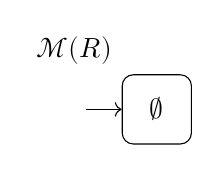
\begin{tikzpicture}
    \tikzset{
      node distance=1cm,
      every state/.style={rectangle, rounded corners, inner sep=0.5em},
      initial text=$ $,
    }
    \node[state, initial, label=above left:$\Automaton{R}$] (u0) {$\Empty$};
  \end{tikzpicture}
\end{center}

\subsection{Prazen niz}

\begin{tcolorbox}[title={Definicija}]
\begin{equation*}
  \begin{aligned}
    R &= \Null\\
    \Language{R} &= \{ \Str{} \}
  \end{aligned}
\end{equation*}
\end{tcolorbox}

\begin{tcolorbox}[title={Konstrukcija}]
\begin{equation*}
  \begin{aligned}
    \Pos\Null &\Move \Null\Pos
  \end{aligned}
\end{equation*}
\end{tcolorbox}

\begin{center}
  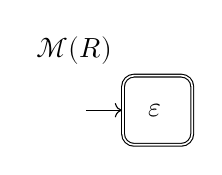
\begin{tikzpicture}
    \tikzset{
      node distance=1cm,
      every state/.style={rectangle, rounded corners, inner sep=0.5em},
      initial text=$ $,
    }
    \node[state, initial, accepting, label=above left:$\Automaton{R}$] (u0) {$\Null\Pos$};
  \end{tikzpicture}
\end{center}

Če $\Str{} \in \Language{r}$, potem rečemo, da je $\RE{R}$ \emph{nullable}.

\subsection{Znak}

\begin{tcolorbox}[title={Definicija}]
\begin{equation*}
  \begin{aligned}
    r &= \Char{a}\text{, kjer } \Char{a} \in \Alphabet\\\
    \Language{r} &= \{ \Str{a} \}
  \end{aligned}
\end{equation*}
\end{tcolorbox}

\begin{tcolorbox}[title={Konstrukcija}]
\begin{equation*}
  \begin{aligned}
    \Pos\Char{a} &\MoveX{\Char{a}} \Char{a}\Pos\\
    %(\RE{R})\Pos &\MoveX{\Char{a}} \RE{R}\\
    \Pos\Char{a} &\MoveX{\Char{b}} \Char{a}\text{, kjer } \Char{a} \neq \Char{b}
  \end{aligned}
\end{equation*}
\end{tcolorbox}

\begin{center}
  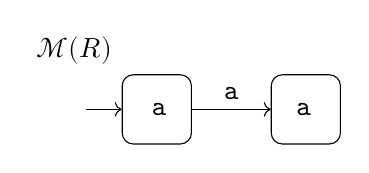
\begin{tikzpicture}
    \tikzset{
      node distance=1cm,
      every state/.style={rectangle, rounded corners, inner sep=0.5em},
      initial text=$ $,
    }
    \node[state, initial, label=above left:$\Automaton{R}$] (u0) {$\Pos\Char{a}$};
    \node[state, right=of u0] (u1) {$\Char{a}\Pos$};
    \draw (u0) edge[->] node[auto]{$\Char{a}$} (u1);
  \end{tikzpicture}
\end{center}

%\begin{equation*}
%  \begin{aligned}
%    \Pos\Set{S} &\MoveX{\Set{S}} \Set{S}\Pos\\
%    %(\RE{R})\Pos &\MoveX{\Char{a}} \RE{R}\\
%    \Pos\Set{S} &\MoveX{\Set{S}} \Set{S}
%  \end{aligned}
%\end{equation*}
%
%\begin{center}
%  \begin{tikzpicture}
%    \tikzset{
%      node distance=1cm,
%      every state/.style={rectangle, rounded corners, inner sep=0.5em},
%      initial text=$ $,
%    }
%    \node[state, initial, label=above left:$\Automaton{R}$] (u0) {$\Pos\Set{S}$};
%    \node[state, right=of u0] (u1) {$\Set{S}\Pos$};
%    \draw (u0) edge[->] node[auto]{$\Set{S}$} (u1);
%  \end{tikzpicture}
%\end{center}

\subsection{Konkatenacija}
\Reset

\begin{tcolorbox}[title={Definicija}]
\begin{equation*}
  \begin{aligned}
  r &= s \Seq t = s \Spc t\\
  \Language{r} &= \{ u \Seq v \mid u \in \Language{s} \land v \in \Language{t}\}
  \end{aligned}
\end{equation*}
\end{tcolorbox}

\begin{tcolorbox}[title={Pravila}]
\begin{equation*}
  \begin{aligned}
  s \Seq t &\not= t \Seq s\\
  s \Seq \Null &= s \\
  \Null \Seq s &= s   \\
  s \Seq \Empty &= \Empty \\
  \Empty \Seq s &= \Empty \\
  (s \Seq p) \Seq q &= s \Seq (p \Seq q) = s \Seq p \Seq q
  \end{aligned}
\end{equation*}
\end{tcolorbox}

\vspace{1em}
\Special{Poseben primer:} Če $|\Language{s}| = |\Language{t}| = 1$, potem $\Language{s} = \{u\}$ in $\Language{t} = \{v\}$ in $\Language{r} = \{u \Seq v\}$.

\Ex
\begin{align*}
  \Language{s} &= \{\Str{Hello}\}\\
  \Language{t} &= \{\Str{World}\}\\
  \Language{r} &= \{\Str{HelloWorld}\}
\end{align*}

Splošno je jezik konkatenacije podoben kartezičnemu produktu.
\begin{align*}
  S &= P \times Q \\
  S &= \{ (x, y) \mid x \in P \land y \in Q\}
\end{align*}

\Ex
\begin{align*}
  P &= \{1, 2, 3\}\\
  Q &= \{a, b\}\\
  S &= \{(1, a), (1, b), (2, a), (2, b), (3, a), (3, b) \}
\end{align*}

Edina razlika je da zamenjamo vsak $(u, v)$, kjer $u \in \Language{s}$ in $v\in \Language{t}$, z $u \Seq v \in \Language{r}$.

\Ex

\begin{align*}
  P &= \{\Str{Dober}, \Str{Lep}\}\\
  Q &= \{\Str{Dan}, \Str{Večer}, \Str{Tek}\}\\
  S &= \{\Str{DoberDan}, \Str{DoberVečer}, \Str{DoberTek}, \Str{LepDan}, \Str{LepVečer}, \Str{LepTek} \}
\end{align*}

\begin{tcolorbox}[title={Konstrukcija}]
  \begin{equation*}
    \begin{aligned}
      \Pos(\RE{R} \Seq \RE{S}) &\Move (\Pos\RE{R}) \Seq \RE{S}\\
      (\RE{R}\Pos) \Seq \RE{S} &\Move \RE{R} \Seq (\Pos \RE{S})\\
      \RE{R} \Seq (\RE{S} \Pos) &\Move (\RE{R} \Seq \RE{S})\Pos
    \end{aligned}
  \end{equation*}
\end{tcolorbox}

\Ex
\begin{align*}
  \N{R} &= \Char{a} \Spc \Char{b} \\
\end{align*}
\begin{multline*}
  \Pos(\Char{a} \Seq \Char{b}) \Move (\Pos\Char{a}) \Seq \Char{b} \MoveX{\Char{a}}
  (\Char{a}\Pos) \Seq \Char{b} \Move \Char{a} \Seq (\Pos\Char{b}) \MoveX{\Char{b}}
  \Char{a} \Seq (\Char{b}\Pos) \Move (\Char{a} \Seq \Char{b})\Pos
\end{multline*}
\begin{center}
  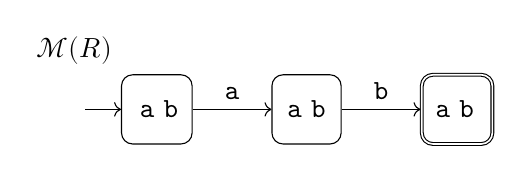
\begin{tikzpicture}
    \tikzset{
      node distance=1cm,
      every state/.style={rectangle, rounded corners, inner sep=0.5em},
      initial text=$ $,
    }

    \node[state, initial, label=above left:$\Automaton{R}$] (u0) {$\Pos\Char{a} \Spc \Char{b}$};
    \node[state, right=of u0] (u1) {$\Char{a} \Pos \Char{b}$};
    \node[state, accepting, right=of u1] (u2) {$\Char{a} \Spc \Char{b}\Pos$};
    \draw (u0) edge[->] node[auto]{\Char{a}} (u1);
    \draw (u1) edge[->] node[auto]{\Char{b}} (u2);
  \end{tikzpicture}
\end{center}

\Ex
\begin{align*}
  \N{R} &= \Char{a} \Spc \Char{b} \Spc \Char{c} \\
\end{align*}
\begin{multline*}
  \Pos((\Char{a} \Seq \Char{b}) \Seq \Char{c}) \Move
  (\Pos(\Char{a} \Seq \Char{b}) \Seq \Char{c}) \Move
  (((\Pos\Char{a}) \Seq \Char{b}) \Seq \Char{c}) \MoveX{\Char{a}}
  (((\Char{a}\Pos) \Seq \Char{b}) \Seq \Char{c}) \Move
  ((\Char{a} \Seq (\Pos \Char{b})) \Seq \Char{c}) \MoveX{\Char{b}}
  ((\Char{a} \Seq (\Char{b}\Pos)) \Seq \Char{c}) \Move\\
  ((\Char{a} \Seq \Char{b})\Pos \Seq \Char{c}) \Move
  ((\Char{a} \Seq \Char{b}) \Seq (\Pos \Char{c})) \MoveX{\Char{c}}
  ((\Char{a} \Seq \Char{b}) \Seq (\Char{c}\Pos)) \Move
  ((\Char{a} \Seq \Char{b}) \Seq \Char{c})\Pos
\end{multline*}
\begin{center}
  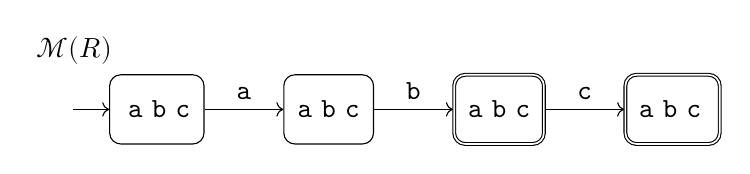
\begin{tikzpicture}
    \tikzset{
      node distance=1cm,
      every state/.style={rectangle, rounded corners, inner sep=0.5em},
      initial text=$ $,
    }

    \node[state, initial, label=above left:$\Automaton{R}$] (u0) {$\Pos\Char{a} \Spc \Char{b} \Spc \Char{c}$};
    \node[state, right=of u0] (u1) {$\Char{a} \Pos \Char{b} \Spc \Char{c}$};
    \node[state, accepting, right=of u1] (u2) {$\Char{a} \Spc \Char{b} \Pos \Char{c}$};
    \node[state, accepting, right=of u2] (u3) {$\Char{a} \Spc \Char{b} \Spc \Char{c}\Pos$};
    \draw (u0) edge[->] node[auto]{\Char{a}} (u1);
    \draw (u1) edge[->] node[auto]{\Char{b}} (u2);
    \draw (u2) edge[->] node[auto]{\Char{c}} (u3);
  \end{tikzpicture}
\end{center}

\subsection*{Primeri}

\subsubsection{"then"}
\begin{equation*}
  \Language{\N{r}} = \{ \Str{then} \}
\end{equation*}

\subsection{Unija}
\Reset

\begin{tcolorbox}[title={Definicija}]
  \begin{equation*}
    \begin{aligned}
    r &= s \Union t \\
      \Language{r} &= \Language{s} \cup \Language{t}
    \end{aligned}
  \end{equation*}
\end{tcolorbox}

\begin{tcolorbox}[title={Pravila}]
  \begin{equation*}
    \begin{aligned}
      s \Union t &= t \Union s \\
      s \Union s &= s \\
      \Empty \Union s &= s \\
      s \Union \Empty &= s \\
      (s \Union p) \Union q &= s \Union (p \Union q) = s \Union p \Union q \\
      s \Seq (p \Union q) &= s \Seq p \Union s \Seq q\\
      (p \Union q) \Seq s &= p \Seq s \Union q \Seq s\\
    \end{aligned}
  \end{equation*}
\end{tcolorbox}

\begin{tcolorbox}[title={Konstrukcija}]
\begin{equation*}
  \begin{aligned}
    \Pos(\RE{R} \Union \RE{S}) &\Move (\Pos\RE{R}) \Union (\Pos\RE{S})\\
    (\RE{R}\Pos) \Union \RE{S} &\Move (\RE{R} \Union \RE{S})\Pos\\
    \RE{R} \Union (\RE{S}\Pos) &\Move (\RE{R} \Union \RE{S})\Pos
  \end{aligned}
\end{equation*}
\end{tcolorbox}

\Ex
\begin{align*}
  \N{R} &= \Char{a} \Union \Char{b} \\
\end{align*}
\begin{equation*}
  \Pos(\Char{a} \Union \Char{b}) \Move
  (\Pos\Char{a}) \Union (\Pos\Char{b}) \begin{aligned}[t]
    &\MoveX{\Char{a}} (\Char{a}\Pos) \Union \Char{b} \Move (\Char{a} \Union \Char{b})\Pos \\
    &\MoveX{\Char{b}} \Char{a} \Union (\Char{b}\Pos) \Move (\Char{a} \Union \Char{b})\Pos \\
  \end{aligned}
\end{equation*}
\begin{center}
  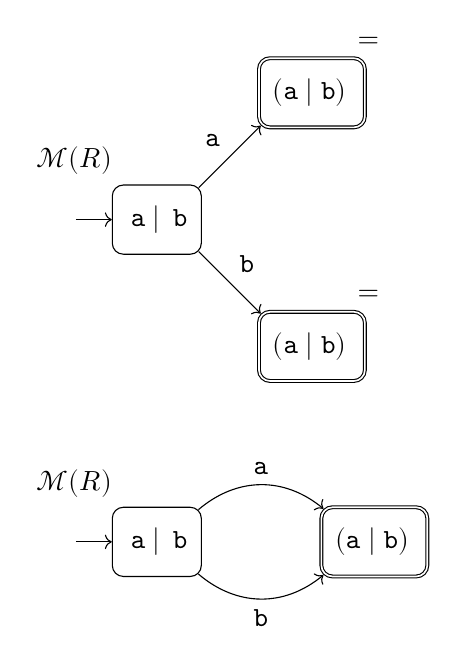
\begin{tikzpicture}
    \tikzset{
      node distance=1cm,
      every state/.style={rectangle, rounded corners, inner sep=0.5em},
      initial text=$ $,
      shorten <>/.style={shorten >=#1, shorten <=#1},
    }

    \node[state, initial, label=above left:$\Automaton{\N{R}}$] (u0) {$\Pos\Char{a} \Union \Pos\Char{b}$};
    \node[state, accepting, above right=of u0, label={above right:=}] (u1) {$(\Char{a} \Union \Char{b})\Pos$};

    \draw (u0.north east) edge[->, shorten <>=-2pt+\pgflinewidth] node[auto]{$\Char{a}$} (u1.south west);

    \node[state, accepting, below right=of u0, label={above right:=}] (u4) {$(\Char{a} \Union \Char{b})\Pos$};

    \draw (u0.south east) edge[->, shorten <>=-2pt+\pgflinewidth] node[auto]{$\Char{b}$} (u4.north west);

    \node[state, initial, below=3.2of u0, label=above left:$\Automaton{\N{R}}$] (p0) {$\Pos\Char{a} \Union \Pos\Char{b}$};
    \node[state, accepting, right=1.5cm of p0] (p1) {$(\Char{a} \Union \Char{b})\Pos$};

    \draw (p0.north east) edge[->, bend left=40, shorten <>=-2pt+\pgflinewidth] node[auto]{$\Char{a}$} (p1.north west);
    \draw (p0.south east) edge[->, bend right=40, shorten <>=-2pt+\pgflinewidth] node[below]{$\Char{b}$} (p1.south west);

  \end{tikzpicture}
\end{center}

\Ex
\begin{align*}
  \N{R} &= \Char{a} \Union \Char{b} \Union \Char{c} \\
\end{align*}
\begin{equation*}
  \Pos((\Char{a} \Union \Char{b}) \Union \Char{c}) \Move
  (\Pos(\Char{a} \Union \Char{b})) \Union (\Pos\Char{c}) \Move
  ((\Pos\Char{a}) \Union (\Pos \Char{b})) \Union (\Pos\Char{c}) \begin{aligned}[t]
    & \MoveX{\Char{a}} ((\Char{a}\Pos) \Union \Char{b}) \Union \Char{c} \Move ((\Char{a} \Union \Char{b}) \Union \Char{c})\Pos \\
    & \MoveX{\Char{b}} (\Char{a} \Union (\Char{b} \Pos)) \Union \Char{c} \Move ((\Char{a} \Union \Char{b}) \Union \Char{c})\Pos \\
    & \MoveX{\Char{c}} (\Char{a} \Union \Char{b}) \Union (\Char{c} \Pos) \Move ((\Char{a} \Union \Char{b}) \Union \Char{c})\Pos 
  \end{aligned}
\end{equation*}

\begin{center}
  \begin{tikzpicture}
    \tikzset{
      node distance=1cm,
      every state/.style={rectangle, rounded corners, inner sep=0.5em},
      initial text=$ $,
      shorten <>/.style={shorten >=#1, shorten <=#1},
    }
    \node[state, initial, below=3.2of u0, label=above left:$\Automaton{\N{R}}$] (p0) {$\Pos\Char{a} \Union \Pos\Char{b} \Union \Pos\Char{c}$};
    \node[state, accepting, right=1.5cm of p0] (p1) {$(\Char{a} \Union \Char{b} \Union \Char{c})\Pos$};

    \draw (p0.north east) edge[->, bend left=40, shorten <>=-2pt+\pgflinewidth] node[auto]{$\Char{a}$} (p1.north west);
    \draw (p0.east) edge[->] node[above]{$\Char{b}$} (p1.west);
    \draw (p0.south east) edge[->, bend right=40, shorten <>=-2pt+\pgflinewidth] node[below]{$\Char{c}$} (p1.south west);
  \end{tikzpicture}
\end{center}

\Ex
\begin{equation*}
  \N{R} = \Char{a} \Spc \Char{b} \Union \Char{a} \Spc \Char{b} \Spc \Char{c} \Union \Char{a} \Spc \Char{c} \Spc \Char{d}
\end{equation*}

\begin{center}
  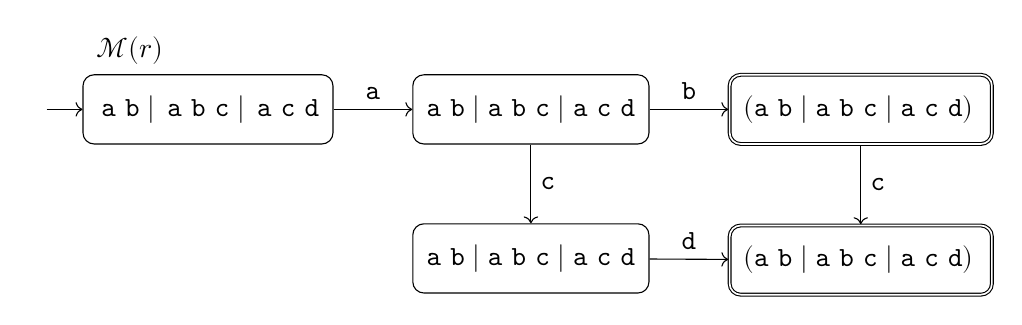
\begin{tikzpicture}
    \tikzset{
      node distance=1cm,
      %every state/.append style={minimum size=0.5cm},
      every state/.style={rectangle, rounded corners, inner sep=0.5em},
      initial text=$ $,
      large/.style={minimum size=1.5cm},
    }

    \node[state, initial, label=above left:$\Automaton{r}$] (u0) {$\Pos\Char{a} \Spc \Char{b} \Union \Pos\Char{a}\Spc\Char{b}\Spc\Char{c} \Union \Pos\Char{a}\Spc\Char{c}\Spc\Char{d}$};
    \node[state, right=of u0] (u1) {$\Char{a} \Pos\Char{b} \Union \Char{a}\Pos\Char{b}\Spc\Char{c} \Union \Char{a}\Pos\Char{c}\Spc\Char{d}$};
    \node[state, accepting, right=of u1] (u2) {$(\Char{a} \Spc\Char{b} \Union \Char{a}\Spc\Char{b}\Pos\Char{c} \Union \Char{a}\Spc\Char{c}\Spc\Char{d})\Pos$};
    \draw (u0) edge[->] node[auto]{$\Char{a}$} (u1);
    \draw (u1) edge[->] node[auto]{$\Char{b}$} (u2);

    \node[state, below=of u1] (u4) {$\Char{a} \Spc\Char{b} \Union \Char{a}\Spc\Char{b}\Spc\Char{c} \Union \Char{a}\Spc\Char{c}\Pos\Char{d}$};
    \node[state, accepting, below=of u2] (u3) {$(\Char{a} \Spc\Char{b} \Union \Char{a}\Spc\Char{b}\Spc\Char{c} \Union \Char{a}\Spc\Char{c}\Spc\Char{d})\Pos$};

    \draw (u2) edge[->] node[auto]{$\Char{c}$} (u3);
    \draw (u1) edge[->] node[auto]{$\Char{c}$} (u4);
    \draw (u4) edge[->] node[auto]{$\Char{d}$} (u3);
  \end{tikzpicture}
\end{center}

\subsection*{Leva faktorizacija}
Skupno predpono izpostavimo.

\Ex
\begin{align*}
  \N{R} &= \Char{a} \Spc \Char{b} \Union \Char{a} \Spc \Char{b} \Spc \Char{c} \Union \Char{a} \Spc \Char{c} \Spc \Char{d}\\
        &= \Char{a} \Seq (\Char{b} \Union \Char{b} \Spc \Char{c} \Union \Char{c} \Spc \Char{d})\\
        &= \Char{a} \Seq (\Char{b} \Seq (\Null \Union \Char{c}) \Union \Char{c} \Spc \Char{d})
\end{align*}

\subsection*{Primeri}
\subsubsection{Ključne besede}

\begin{equation*}
  \N{R} = \Char{i} \Spc \Char{f} \Union \Char{f} \Spc \Char{o} \Spc \Char{r} \Union \Char{f} \Spc \Char{o} \Spc \Char{r} \Spc \Char{e} \Spc \Char{a} \Spc \Char{c} \Spc \Char{h}
\end{equation*}

Avtomat je optimalen.
Ne vemo za katero ključno besedo smo našli ujemanje.

\subsection{Množica znakov}
\Reset

\begin{tcolorbox}[title={Definicija}]
\begin{equation*}
  \begin{aligned}
    r &= S\text{, kjer } S \subseteq \Alphabet \\
    &= \Char{a} \Union \dots \Union \Char{b}\text{, kjer } \Char{a}, \dots, \Char{b} \in S\\
    \Language{r} &= S
  \end{aligned}
\end{equation*}
\end{tcolorbox}

    %\node[state, initial, below=2of p0, label=above left:$\Automaton{\N{r}}$] (q0) {$\Pos\Char{a} \Union \Pos\Char{b}$};
    %\node[state, accepting, right=2.5cm of q0] (q1) {$(\Char{a} \Union \Char{b})\Pos$};
%
%    \draw (q0) edge[->] node[auto]{$\{\Char{a}, \Char{b}\}$} (q1);
%
%
%  \end{tikzpicture}
%\end{center}

\subsection{Opcija}
\Reset

\begin{tcolorbox}[title={Definicija}]
  \begin{equation*}
    \begin{aligned}
      \Opt{S} &= \Null \Union s\\
      \Language{\Opt{S}} &= \{\Str{}\} \cup \Language{s}
    \end{aligned}
  \end{equation*}
\end{tcolorbox}

Ujemanje $S$ 0 ali 1 krat.

\begin{tcolorbox}[title={Konstrukcija}]
\begin{equation*}
  \begin{aligned}
    \Pos(\Opt{\RE{R}}) &\Move (\Opt{(\Pos\RE{R})})\Pos\\
    \Opt{(\RE{R}\Pos)} &\Move (\Opt{\RE{R}})\Pos
  \end{aligned}
\end{equation*}
\end{tcolorbox}

\begin{center}
  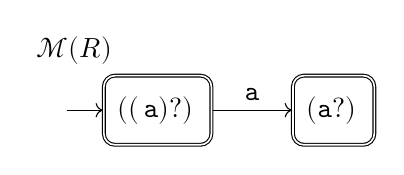
\begin{tikzpicture}
    \tikzset{
      node distance=1cm,
      every state/.style={rectangle, rounded corners, inner sep=0.5em},
      initial text=$ $,
    }
    \node[state, initial, accepting, label=above left:$\Automaton{R}$] (u0) {$(\Opt{(\Pos\Char{a})})\Pos$};
    \node[state, accepting, right=of u0] (u1) {$(\Opt{\Char{a}})\Pos$};
    \draw (u0) edge[->] node[auto]{$\Char{a}$} (u1);
  \end{tikzpicture}
\end{center}

\subsection{Potence}
\Reset

\begin{tcolorbox}[title={Definicija}]
\begin{equation*}
  \begin{aligned}
    \Rep{s}{0} &= \Null\\
    \Rep{s}{i+1} &= \Rep{s}{i} \Seq s\\[1em]
    \Rep{s}{i} &= \underbrace{s \Seq \ldots \Seq s}_{i}\\[1em]
    \Language{\Rep{s}{0}} &= \Null\\
    \Language{\Rep{s}{i+1}} &= \{u \Seq v \mid u \in \Language{\Rep{s}{i}} \land v \in \Language{s}\}
  \end{aligned}
\end{equation*}
\end{tcolorbox}
\begin{align*}
\end{align*}

\begin{tcolorbox}[title={Konstrukcija}]
\begin{equation*}
  \begin{aligned}
    \Pos(\Rep{\RE{R}}{n}) &\Move \Rep{(\Pos\RE{R})}{n}\\
    \Rep{(\RE{R}\Pos)}{n} &\Move \Rep{(\Pos\RE{R})}{n-1}\\
    \Rep{(\Pos\RE{R})}{0} &\Move (\Rep{\RE{R}}{0})\Pos
  \end{aligned}
\end{equation*}
\end{tcolorbox}

\begin{center}
  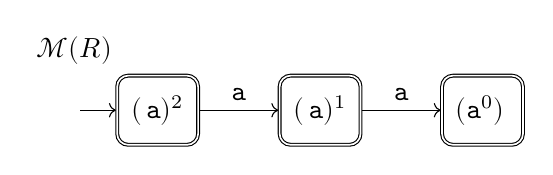
\begin{tikzpicture}
    \tikzset{
      node distance=1cm,
      every state/.style={rectangle, rounded corners, inner sep=0.5em},
      initial text=$ $,
    }
    \node[state, initial, accepting, label=above left:$\Automaton{R}$] (u0) {$(\Pos\Char{a})^2$};
    \node[state, accepting, right=of u0] (u1) {$(\Pos\Char{a})^1$};
    \node[state, accepting, right=of u1] (u2) {$(\Char{a}^0)\Pos$};
    \draw (u0) edge[->] node[auto]{$\Char{a}$} (u1);
    \draw (u1) edge[->] node[auto]{$\Char{a}$} (u2);
  \end{tikzpicture}
\end{center}

\subsection{Kleene-ovo zaprtje}
\Reset

\begin{tcolorbox}[title={Definicija}]
  \begin{equation*}
    \begin{aligned}
      \Kleene{s} &= \Null \Union s \Union s \Seq s \Union s \Seq s \Seq s \Union \ldots \\
      &= \Rep{s}{0} \Union \Rep{s}{1} \Union \Rep{s}{2} \Union \ldots \\
      &= \Big\vert_{i = 0}^\infty \Rep{s}{i}\\
      \Language{\Kleene{s}} &= \bigcup_{i = 0}^\infty \Language{s^i}
    \end{aligned}
  \end{equation*}
\end{tcolorbox}

Ujemanje $s$ 0 ali več krat.
Z drugimi besedami, $s$ je lahko ponovljen $0, 1, 2, \dots, \infty$ krat.

\begin{tcolorbox}[title={Pravila}]
  \begin{equation*}
    \begin{aligned}
      \Kleene{\Empty} &= \Null\\
      \Kleene{\Null} &= \Null\\
      \Null \Union \Kleene{s} &= \Kleene{s}\\
      \Kleene{s} \Union \Null &= \Kleene{s}\\
      \Kleene{(\Kleene{s})} &= \Kleene{s}\\
      \Kleene{(s \Union t)} &= \Kleene{(\Kleene{s} \Seq t)} \Seq \Kleene{s}\\
      \Kleene{(s \Seq t)} &= \Null \Union s \Seq \Kleene{(t \Seq s)} \Seq t\\
      \Kleene{s} &= (\Null \Union s \Union ... \Union \Rep{s}{i - 1}) \Seq \Kleene{(\Rep{s}{i})}
    \end{aligned}
  \end{equation*}
\end{tcolorbox}

\begin{tcolorbox}[title={Konstrukcija}]
\begin{equation*}
  \begin{aligned}
    \Pos(\Kleene{\RE{R}}) &\Move (\Kleene{(\Pos\RE{R})})\Pos\\
    \Kleene{(\RE{R}\Pos)} &\Move (\Kleene{(\Pos\RE{R})})\Pos
  \end{aligned}
\end{equation*}
\end{tcolorbox}

\begin{center}
  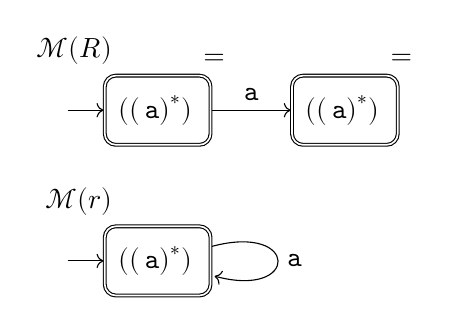
\begin{tikzpicture}
    \tikzset{
      node distance=1cm,
      every state/.style={rectangle, rounded corners, inner sep=0.5em},
      initial text=$ $,
    }
    \node[state, initial, accepting, label=above left:$\Automaton{R}$, label={above right:=}] (u0) {$(\Kleene{(\Pos\Char{a})})\Pos$};
    \node[state, accepting, right=of u0, label={above right:=}] (u1) {$(\Kleene{(\Pos\Char{a})})\Pos$};
    \draw (u0) edge[->] node[auto]{$\Char{a}$} (u1);

    \node[state, initial, below=of u0, accepting, label=above left:$\Automaton{r}$] (p0) {$(\Kleene{(\Pos\Char{a})})\Pos$};
    \draw (p0) edge[->, loop right] node[auto]{$\Char{a}$} (p0);
  \end{tikzpicture}
\end{center}

\subsection{Pozitivno zaprtje}
\Reset

\begin{tcolorbox}[title={Definicija}]
  \begin{equation*}
    \begin{aligned}
      \KleenePlus{s} &= s \Union s \Seq s \Union s \Seq s \Seq s \Union \ldots \\
      &= \Rep{s}{1} \Union \Rep{s}{2} \Union \ldots \\
      &= \Big\vert_{i = 1}^\infty \Rep{s}{i}\\
      \Language{\KleenePlus{s}} &= \bigcup_{i = 1}^\infty \Language{s^i}\\[1em]
      \Kleene{s} &= \Null \Union \KleenePlus{s} = \Opt{(\KleenePlus{s})} = \KleenePlus{(\Opt{s})}\\
      \Language{\Kleene{r}} &= \{\Str{}\} \cup \Language{\KleenePlus{r}}
    \end{aligned}
  \end{equation*}
\end{tcolorbox}

Ujemanje $s$ 1 ali več krat.
Z drugimi besedami, $s$ je lahko ponovljen $1, 2, \dots, \infty$ krat.

\begin{equation*}
  \begin{aligned}
    \Pos(\KleenePlus{\RE{R}}) &\Move \KleenePlus{(\Pos\RE{R})}\\
    \KleenePlus{(\RE{R}\Pos)} &\Move (\KleenePlus{(\Pos\RE{R})})\Pos
  \end{aligned}
\end{equation*}

\begin{center}
  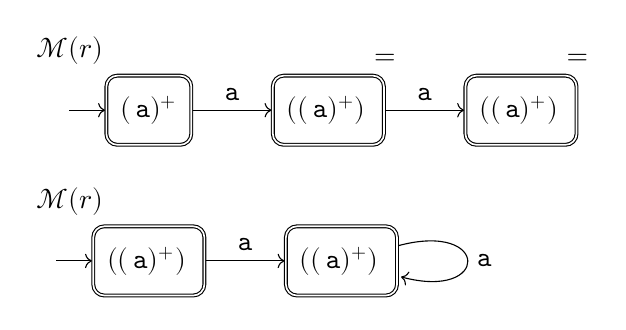
\begin{tikzpicture}
    \tikzset{
      node distance=1cm,
      every state/.style={rectangle, rounded corners, inner sep=0.5em},
      initial text=$ $,
    }
    \node[state, initial, accepting, label=above left:$\Automaton{r}$] (u0) {$\KleenePlus{(\Pos\Char{a})}$};
    \node[state, accepting, right=of u0, label={above right:=}] (u1) {$(\KleenePlus{(\Pos\Char{a})})\Pos$};
    \node[state, accepting, right=of u1, label={above right:=}] (u2) {$(\KleenePlus{(\Pos\Char{a})})\Pos$};
    \draw (u0) edge[->] node[auto]{$\Char{a}$} (u1);
    \draw (u1) edge[->] node[auto]{$\Char{a}$} (u2);

    \node[state, initial, below=of u0, accepting, label=above left:$\Automaton{r}$] (p0) {$(\KleenePlus{(\Pos\Char{a})})\Pos$};
    \node[state, accepting, right=of p0] (p1) {$(\KleenePlus{(\Pos\Char{a})})\Pos$};
    \draw (p0) edge[->] node[auto]{$\Char{a}$} (p1);
    \draw (p1) edge[->, loop right] node[auto]{$\Char{a}$} (p1);
  \end{tikzpicture}
\end{center}

\subsection*{Primeri}
\subsubsection{Števila}
\begin{equation*}
  \N{R} = \KleenePlus{\{\Char{0}, \dots, \Char{9}\}}
\end{equation*}
\Next

\subsubsection{Naravna števila}
\begin{equation*}
  \Language{\N{r}} = \{\Str{1}, \Str{2}, \dots\}
\end{equation*}
\Next

\subsubsection{Cela števila}
\begin{align*}
  \N{s} &= \{\Char{0}, \dots, \Char{9}\} \\
  \N{r} &= (\Char{+} \Union \Char{-}) \Seq \KleenePlus{\N{s}}
\end{align*}
\Next

\subsubsection{Heksadecimalna števila}
\begin{equation*}
  \Language{\N{r}} = \{\Str{0x0}, \Str{0x1}, \dots, \Str{0xA}, \dots, \Str{0xFFFF}, \dots\}
\end{equation*}
\Next

\subsubsection{Barve}
\begin{equation*}
  \Language{\N{r}} = \{\Str{\#000000}, \dots, \Str{\#FFFFFF}\}
\end{equation*}
\Next

\subsubsection{Števila s plavajočo vejico}
\begin{align*}
  \N{s} &= \{\Char{0}, \dots, \Char{9}\} \\
  \N{r} &= (\Char{+} \Union \Char{-}) \Seq \KleenePlus{\N{s}} \Spc \Char{.} \Spc \Kleene{\N{s}}
\end{align*}
\Next

\subsubsection{Imena spremenljivk}
\begin{align*}
  \N{l} &= \{\Char{a}, \dots, \Char{z}\} \\
  \N{r} &= \KleenePlus{\N{l}}
\end{align*}


\subsubsection{Ključne besede in imena spremenljivk}
\begin{align*}
  \N{i} &= \KleenePlus{\{\Char{a}, \dots, \Char{z}\}}\\
  \N{k} &= \Char{a} \Spc \Char{b} \Union \Char{a} \Spc \Char{b} \Spc \Char{c} \Union \Char{a} \Spc \Char{c} \Spc \Char{d}\\
  \N{r} &= \N{i} \Union \N{k}
\end{align*}


\end{document}
